% \documentclass[10pt,a4paper,spanish, twocolumn]{report}

% % a4large.sty -- fill an A4 (210mm x 297mm) page
% % Note: 1 inch = 25.4 mm = 72.27 pt
% %       1 pt   =  3.5 mm (approx)

% % vertical page layout -- one inch margin top and bottom
% \topmargin        0   mm    % top margin less 1 inch
% \headheight       0   mm    % height of box containing the head
% \headsep          0   mm    % space between the head and the body of the page
% \textheight     240   mm    % the height of text on the page
% \footskip         7   mm    % distance from bottom of body to bottom of foot

% % horizontal page layout -- one inch margin each side
% \oddsidemargin    0   mm    % inner margin less one inch on odd pages
% \evensidemargin   0   mm    % inner margin less one inch on even pages
% \textwidth      159.2 mm    % normal width of text on page

% \usepackage[utf8]{inputenc}
% \usepackage[%english
%             spanish
%            ]
%            {babel}
% \usepackage[usenames,dvipsnames]{color}
% %\usepackage{chessboard}
% \usepackage[pdftex]{graphicx}
% \usepackage{amsmath,amsthm,latexsym}
% \usepackage{amsfonts,amssymb}
% \usepackage{enumerate}
% \usepackage{subfigure}
% \usepackage{minted}
% \usepackage{tikz}
% \usepackage{pgfplots}

% \usepackage[bookmarks=true,
%             bookmarksnumbered=false, % true means bookmarks in 
%                                      % left window are numbered                         
%             bookmarksopen=false,     % true means only level 1
%                                      % are displayed.
%             colorlinks=true,
%             linkcolor=webred]{hyperref}
% \definecolor{webgreen}{rgb}{0, 0.5, 0} % less intense green
% \definecolor{webblue}{rgb}{0, 0, 0.5}  % less intense blue
% \definecolor{webred}{rgb}{0.5, 0, 0}   % less intense red
% \definecolor{dblackcolor}{rgb}{0.0,0.0,0.0}
% \definecolor{dbluecolor}{rgb}{.01,.02,0.7}
% \definecolor{dredcolor}{rgb}{0.8,0,0}
% \definecolor{dgraycolor}{rgb}{0.30,0.3,0.30}

% %%    macro tomada de clogica.tex

%  \newcommand{\regla}[2]{
%    \begin{array}{c}
%      #1\\
%      \hline
%      #2\\
%    \end{array}
%  }

% \newcommand*{\textcal}[1]{
%              % family qzc: Font TeX Gyre Chorus (package tgchorus)
%              % family pzc: Font Zapf Chancery (package chancery)
%              \textit{\fontfamily{pzc}\selectfont#1}
%                          }

% \newenvironment{parrafo}{\begin{trivlist}\item []}{\end{trivlist}}
% %\renewcommand{\baselinestretch}{1.5}

% \renewcommand{\labelitemii}{$\ast$}
% %\renewcommand{\labelitemii}{$\cdot$}
% \renewcommand{\labelitemiii}{$\diamond$}
% \renewcommand{\labelitemiv}{$\bullet$}

% %%%%%%%%%% English %%%%%%%%%

% \newtheorem{theorem}{Theorem}[section]
% \newtheorem{corollary}[theorem]{Corollary}
% \newtheorem{lemma}[theorem]{Lemma}
% \newtheorem{proposition}[theorem]{Proposition}
% \newtheorem{example}[theorem]{Ejemplo}
% \newtheorem{ax}{Axiom}
% \newtheorem{algoritmo}[theorem]{Algorithm}

% \theoremstyle{definition}
% \newtheorem{definition}{Definition}[section]

% \theoremstyle{remark}
% \newtheorem{remark}{Remark}[section]
% \newtheorem*{notation}{Notación}

% %\numberwithin{equation}{section}

% %%%%%%%%%%%%%%%%%%%%%%%%%%%%%%%%%

% %%%%% Para cambiar el tipo de letra en el título de la sección %%%%%%%%%%%
% \usepackage{sectsty}
% \chapterfont{\fontfamily{pag}\selectfont} %% for chapter if you want
% \sectionfont{\fontfamily{pag}\selectfont}
% \subsectionfont{\fontfamily{pag}\selectfont} 
%             %% Similarly for others. see the manual of sectsty, section 5.
% %%%%%%%%%%%%%%%%%%%%%%%%%%%%%%%%%%%%%%%%%%%%%%%%%%%%%%%%%%%%%%%%%%%%%%%%%%
\begin{twocolumn}

% \title{Tema 2: Ejemplos de eficiencias}
% \author{Braulio Vargas López y Marta Gómez Macías}
% \date{\today}
% \maketitle

\subsection{$3n^2 \in O(n^2)$}

Aplicamos la condición de O-grande
\begin{displaymath}
3n^2 \leq c \cdot n^2
\end{displaymath}
Como necesitamos saber el valor exacto de n, lo igualamos
\begin{displaymath}
3n^2 = c \cdot n^2
\end{displaymath}
\begin{displaymath}
3n^2 - c \cdot n^2 = 0
\end{displaymath}
\begin{displaymath}
n^2 \cdot (3 - c) = 0
\end{displaymath}
\begin{displaymath}
n^2 = \frac{0}{3 - c}
\end{displaymath}
Obtenemos como valor de $n$ el cero y como valor de c, un valor que cumpla la condición de ser menor que tres.
\begin{displaymath}
n = 0, c < 3
\end{displaymath}

\subsection{$3n^2 \in \Omega(n^2)$}

Aplicamos la definición de $\Omega$
\begin{displaymath}
3n^2 \geq c \cdot n^2
\end{displaymath}
Igualamos para obtener el valor exacto
\begin{displaymath}
3n^2 \leq c \cdot n^2
\end{displaymath}
\begin{displaymath}
3n^2 = c \cdot n^2
\end{displaymath}
\begin{displaymath}
3n^2 - c \cdot n^2 = 0
\end{displaymath}
\begin{displaymath}
n^2 \cdot (3 - c) = 0
\end{displaymath}
\begin{displaymath}
n^2 = \frac{0}{3 - c}
\end{displaymath}
Obtenemos como valor de $n$ el cero y como valor de c, un valor que cumpla la condición de ser menor que tres.
\begin{displaymath}
n = 0, c < 3
\end{displaymath}

\subsection{$3n^2 \in \Theta(n^2)$}


Como en los dos casos anteriores se cumple la condición, $3n^2 \in \Theta(n^2)$ es cierto en este caso.

\subsection{$2^{n+1} \in O(2^n)$}

\begin{displaymath}
2^{n+1} \leq c \cdot 2^{n}
\end{displaymath}
Vamos a realizar un cambio de variable para despejar la constante $c$
\begin{displaymath}
m = 2^n \qquad 2 \cdot m = c \cdot m
\end{displaymath}
\begin{displaymath}
2 = c
\end{displaymath}
La constante de la función será 2 en este caso, y ahora vamos a calcular el valor de $n$, sustituyendo $c$ por su valor.
\begin{displaymath}
2^{n+1} = 2 \cdot 2^n
\end{displaymath}
\begin{displaymath}
n = 0
\end{displaymath}

\subsection{$O(n) \in O(n^2)$}

Realizamos el límite entre ambas funciones:
\begin{displaymath}
\lim_{n \rightarrow \infty} \frac{n}{n^2} = 0
\end{displaymath}
Como sale cero, nos fijamos en la regla de relación límites/órdenes que dice que
\begin{displaymath}
\lim_{n \rightarrow \infty} \frac{f(n)}{g(n)} \Longrightarrow O(f) \subset O(g)
\end{displaymath}
Y en la regla de relación pertenencia/contenido que dice que
\begin{displaymath}
O(f) \subseteq O(g) \Longleftrightarrow f \in O(g)
\end{displaymath}
Y concluímos que $O(n)$ está incluído en $O(n^2)$.

\subsection{$n^2 \in O(n^3)$}


Siguiendo las reglas de O-grande, $n^2$ está incluido en $O(n^3)$.

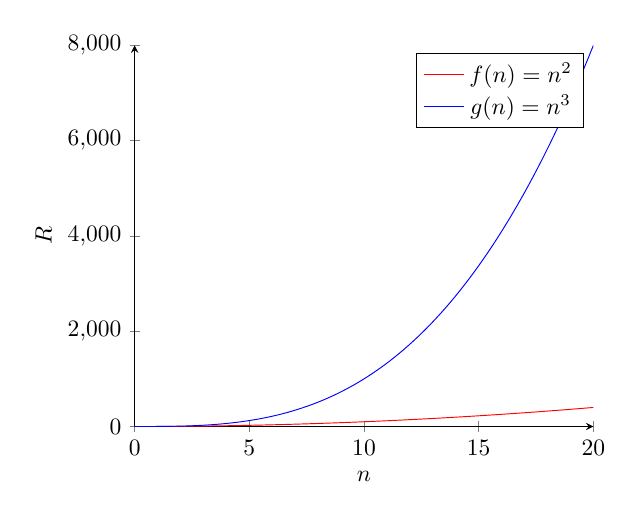
\begin{tikzpicture}[scale=0.85]
\begin{axis}[
    axis lines = left,
    xlabel = $n$,
    ylabel = {$R$},
]
%Below the red parabola is defined
\addplot [
    domain=0:20,
    samples=100,
    color=red,
]
{x^2};
\addlegendentry{$f(n)=n^{2}$}
%Here the blue parabloa is defined
\addplot [
    domain=0:20,
    samples=100,
    color=blue,
    ]
    {x^3};
\addlegendentry{$g(n)=n^3$}

\end{axis}
\end{tikzpicture}

\subsection{$n^2 \in \Omega(n^3)$}

Como se ve en la gráfica anterior, $n^3$ está muy por encima de $n^2$. Además, si aplicamos la definición de $\Omega$ obtenemos que:
\begin{displaymath}
n^2 \geq c \cdot n^3
\end{displaymath}
\begin{displaymath}
n^2 = c \cdot n^3
\end{displaymath}
¿Por qué valor $c$ multiplicamos $n^3$ para que se convierta en $n^2$?

\subsection{$n^2 \in \Theta(n^3)$}


Como $n^2 \in \Omega(n^3)$ no es cierto, $n^2 \in \Theta(n^3)$ no puede estar incluido en el orden exacto de $n^3$.

\subsection{$(2 + 1)^n \in O(2^n)$}
\label{apartado9}


Es imposible por la siguiente razón

\begin{displaymath}
\lim_{n \rightarrow \infty} \frac{3^n}{2^n} = +\infty
\end{displaymath}

\subsection{$(n+1)! \in O(n!)$}

Al igual que la anterior, no está incluida
\begin{displaymath}
\lim_{n \rightarrow \infty} \frac{(n+1)!}{n!} = +\infty
\end{displaymath}

\subsection{$n^3 \in O(n^2)$}


Si calculamos el límite cuando $n$ tiene a infinito, el resultado de este límite es infinito, por lo que $n^3 \notin O(n^2)$

\begin{displaymath}
\lim_{n \rightarrow \infty} \frac{n^3}{n^2} = +\infty
\end{displaymath}

\subsection{$n^3 \in \Omega(n^2)$}


Como vimos en el apartado anterior, $n^3$ tiene una velocidad de crecimiento mucho mayor que $n^2$, por lo que si $n^3$ no está contenido en $O(n^2)$ es imposible que esté contenido en $\Omega(n^2)$, por lo que $n^3 \notin \Omega(n^2)$

% \begin{displaymath}

% \end{displaymath}

\subsection{$n^3 \in \Theta(n^2)$}


Como $n^3 \notin O(n^2)$ y $n^3 \notin \Omega(n^2)$, $n^3 \notin \Theta(n^2)$ porque estos valores no se incluyen en la intersección de $O(n^2)$ y $\Omega(n^2)$
% \begin{displaymath}

% \end{displaymath}

\subsection{$(2+1)^n \in \Omega(2^n)$}


Como se vio en el \hyperref[apartado9]{apartado \ref*{apartado9}}, $(2+1)^n \notin O(2^n)$, por lo que tampoco estará incluido en el mejor caso, es decir, $(2+1)^n \notin \Omega(2^n)$
% \begin{displaymath}

% \end{displaymath}

\subsection{$n^2 \in O(n!!)$}


Para comprobar si la inclusión es cierta, vamos a realizar el límite cuando $n$ tiende a $\infty$.

\begin{displaymath}
  \lim_{n \rightarrow \infty} \frac{n^2}{n!!} = 0
\end{displaymath}

Como vemos, el resultado es 0, por lo que $n^2 \in O(n!!)$ es cierto.

\end{twocolumn} 
\hyperref[apartado9]{apartado \ref*{apartado9}}